
\subsection{Electron reconstruction}

Electrons and photons appear in many interesting final states,
including Higgs decay chains, making it crucial to efficiently
reconstruct these particles. In the ATLAS detector, an electron is
loosely defined as energy deposits in the EM calorimeter matched to a
reconstructed track. Sliding window clustering, described in
section~\ref{chap:reconstruction:sec:cluster:subsec:sliding_window},
is used. The efficiency for finding the EM showers associated with a
true electron with sliding window clustering is 95\% at $\et =
7~\gev$, increasing to 99.9\% at $\et =
45~\gev$~\cite{bib:ATLAS-CONF-2014-032}.

Tracks associated with electron candidates are reconstructed with the
algorithms discussed in section~\ref{chap:reco:sec:tracks}, with some
important differences to account for the propensity for electrons to
emit radiation as they pass through matter. Electron track candidates are extended
through the inner detector with the Kalman filter approach. In the
first fit attempt, scattering in the detector material assumes the
particle is a pion. Upon reaching the calorimeter, if the track does
not overlap with a region of interest (ROI), defined as the $\Delta{R}
< 0.3$ region around the center of an EM cluster which satisfies loose
shower shape requirements, then starting from the
track seed, the track is propagated again, instead assuming an
electron-like interaction with the detector material. The electron
hypothesis allows for up to 30\% energy loss due to {\it
  Bremsstrahlung}. All track candidates found to overlap with ROIs are
then re-fitted using the global $\chi^2$ track-fitting algorithm. These
tracks are extrapolated to the middle layer of the EM calorimeter. For
each of these track candidates, one of two requirements must be satisfied:
(1) the track falls within $\phi = 0.2$ in the direction of deflection
and $\phi = 0.05$ in the opposite direction, and within $\eta = 0.05$
of the center of the EM cluster, (2) after rescaling the track
momentum by the measured cluster energy, the track is within $\phi =
0.1$ in the direction of deflection and $\phi = 0.05$ in the other
direction of the center of the EM cluster. These two requirements are
adjusted slightly for track candidates with less than 4 silicon
hits (TRT-only tracks). Requirement (2) is designed to retain low \pt~tracks that may
have suffered significant energy losses before reaching the
calorimeter.

With the exception of TRT-only tracks, tracks that pass either of the requirements are then re-fitted again
with the Gaussian Sum Filter (GSF)
algorithm~\cite{bib:ATLAS-CONF-2012-047}, which is a generalization of
the Kalman filter algorithm that accounts for nonlinear effects from
{\it Bremsstrahlung}. The re-fitted
tracks are matched to EM clusters again, this time with tighter
requirements on the $\Delta{\phi}$ and $\Delta{\eta}$ distances. For
cases in which more than one track is associated to a cluster, tracks
with more pixel hits that fall closer to the cluster center are
favored. 

With tracks matched to clusters, the calorimeter clusters are then
rebuilt in each layer using sliding window dimensions that have been
optimized for electrons. The size of the window is $3 \times 7$ ($5
\times 5$) in the barrel (endcaps). In order to reduce the
uncertainties on the measured energy, a multivariate regression
technique is used to correct for instrumental effects. The regressor,
which has been trained on single electron events, determines a
correction factor for the total cluster energy, using as independent
variables the total energy measured in the calorimeter, the ratio of
the presampler energy to the EM calorimeter energy, the shower depth,
the pseudorapidity of the center of the cluster in the global
coordinate system, and the $\eta$ and $\phi$ of the cluster in the
calorimeter coordinate system~\cite{bib:Aad:2014nim}. The performance
of the MVA technique is summarized in
figure~\ref{chap:reconstruction:fig:elec_mva}. The most
probable value (MPV) of the ratio of the measured energy to the true
energy as a function of $\eta_{\textrm{electron}}$, an
estimate of the linearity of the technique, is less than 0.5\% across
the \et~range in the barrel region, while in the forward calorimeter
the effect is slightly larger due to more detector material in front
of the calorimeter. Similarly, the relative energy resolution ($\sigma/E$) grows
with $|\eta|$ due to material effects. 

\begin{figure}[ht]
    \centering
    \subfigure{
    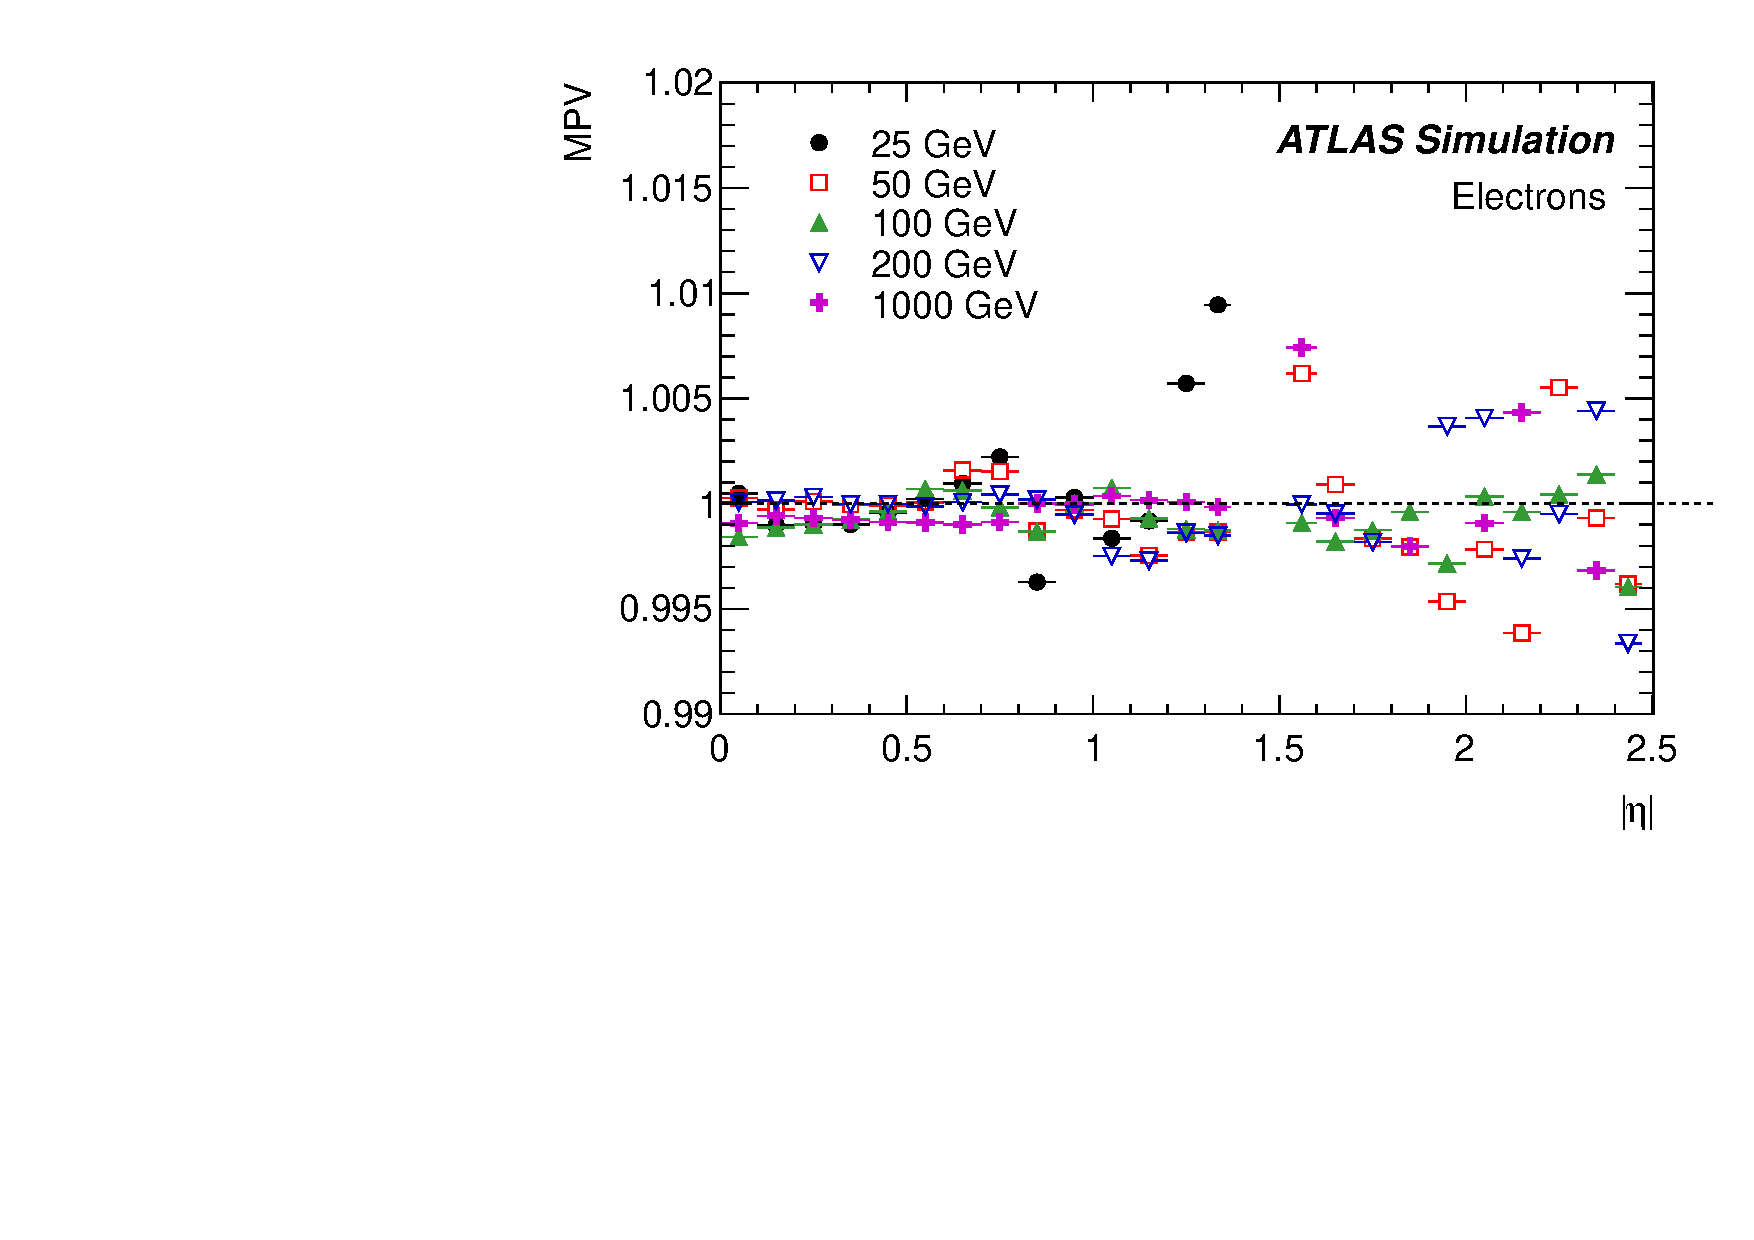
\includegraphics[width=0.4\textwidth]{fig/reconstruction/elec_mva_EdivEtrue.pdf}
    \label{chap:reconstruction:fig:elec_mva_EdivEtrue}
    }
    \subfigure{
    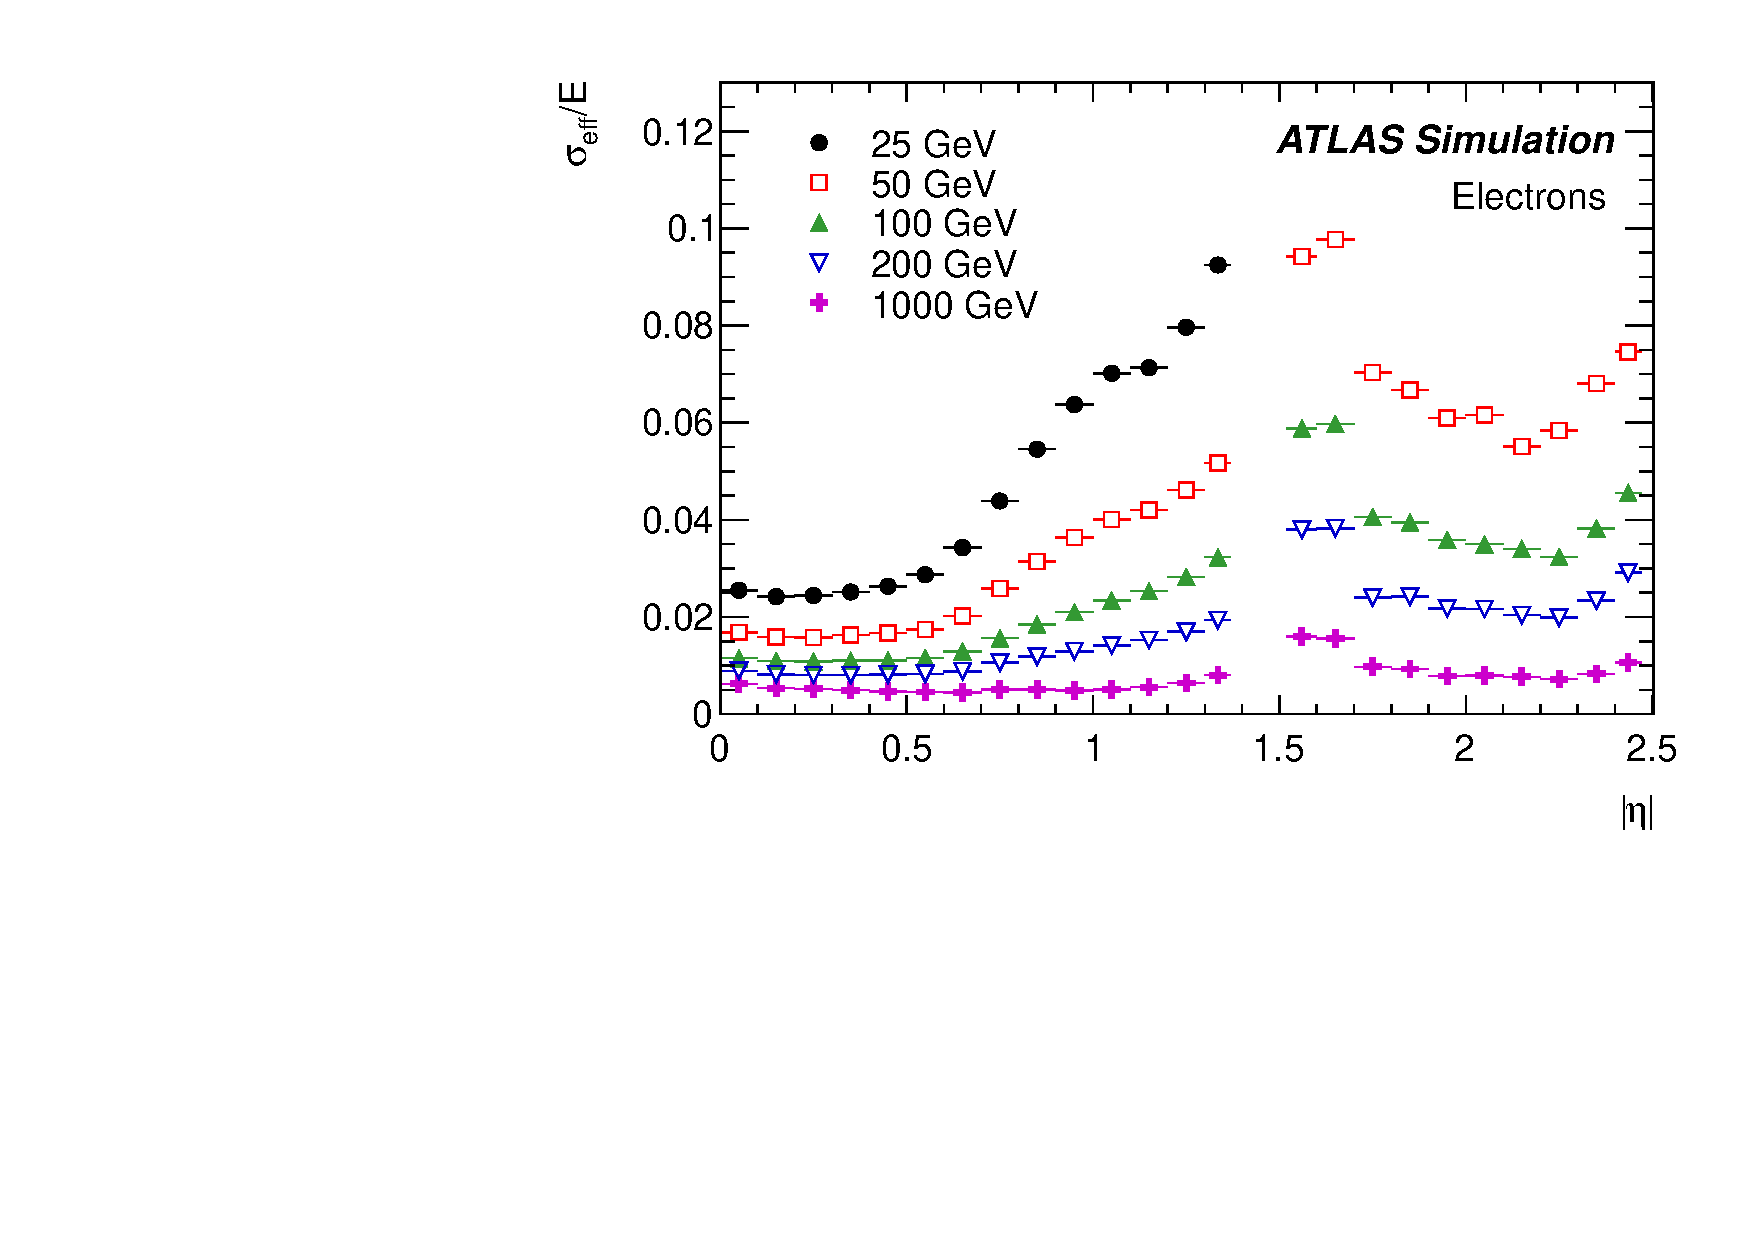
\includegraphics[width=0.4\textwidth]{fig/reconstruction/elec_mva_resolution.pdf}
    \label{chap:reconstruction:fig:elec_mva_resolution}
    }
    \caption[]{The most-probable-value (MPV) of the ratio of the
      measured energy to the true
      energy~\subref{chap:reconstruction:fig:elec_mva_EdivEtrue} and
      the energy
      resolution~\subref{chap:reconstruction:fig:elec_mva_resolution}
      as a function of $\eta_{\textrm{electron}}$ for electrons of
      various \pt.~\cite{bib:Aad:2014nim}}
\label{chap:reconstruction:fig:elec_mva}
\end{figure}

The 4-momentum of the reconstructed electron candidate is derived from
both calorimeter and track information. The electron energy is taken
from the calorimeter cluster, while the $\eta$ and $\phi$ are taken from
the best-matched track. For TRT-only tracks, $\eta$ and $\phi$ from
the cluster are used. 

\subsection{Electron identification}

Electrons which are reconstructed according to the algorithm described
in the previous section can arise from backgrounds, including charged
hadrons, semi-leptonic heavy flavor hadron decays, the Dalitz decay of the pion ($\pi_0
\rightarrow{e^+ e^- \gamma}$), and photon conversions. To suppress
these backgrounds while retaining true prompt electrons, candidates are
identified using a collection of discriminating variables, either
placing sequential cuts on the variables, or using them as inputs to a
multivariate algorithm. In the tracking region ($\eta < 2.47$), signal
and background electrons are distinguished by variables which describe the
EM shower shapes, properties of tracks, as well as the
matching between the track and EM cluster~\cite{bib:ATLAS-CONF-2014-032}. 

Cut-based electron identification cut criteria are categorized based
on the rejection power. In order of increasing rejection-- and decreasing
efficiency-- the categories are called {\it loose}, {\it medium}, and
{\it tight}. Electrons selected with the {\it tight} criteria are a
subset of {\it loose} and {\it medium}, and those selected with {\it
  medium} are a subset of {\it loose}. These selection criteria have
been optimized in bins of electron \et~and $\eta$ to account for the
fact that shower shapes vary with these quantities. 

To improve on the cut-based identification approach, the same
discriminating variables are used in a likelihood-based multivariate
technique. The electron likelihood is defined by the equation

\begin{equation}
L_{s(b)}(\vect{x}) = \prod_{i=1}^n P_{s(b),i}(x_i)
\end{equation}

\noindent
where $P_{s(b),i}(x_i)$ is the signal (background) probability
density function (p.d.f.) for the $i^{\textrm{th}}$ variable evaluated at
$x_i$. The p.d.f.s are obtained from data in control regions. Track
hit requirements are not included in the likelihood and are instead
left as cuts. As in cut-based electron identification, there are three
selection categories based on background rejection. The
\textsc{loose}, \textsc{medium}, and \textsc{very tight} categories
correspond to different cuts on the likelihood-based discriminant
$L_s/(L_s+L_b)$, and the cut values are chosen such that the
efficiencies are approximately the same those of the corresponding
cut-based categories. In addition to different discriminant
cut-values, each likelihood category uses a different set of input
variables in the likelihood. The \textsc{loose} category features
variables that are efficient in rejecting electron candidates in
light-flavor jets, while \textsc{medium} and \textsc{very tight}
include additional variables that help in the discrimination against
heavy flavor jets and photon conversions. The p.d.f.s that define the
likelihood are subdivided into nine $|\eta|$ bins and six \et~bins
whose boundaries roughly correspond to those in cut-based
identification. Due to limited data statistics, however, the binning
is coarser for likelihood-based electron identification.

In addition to the identification requirements above, hadronic
backgrounds are further rejected by requiring that the electron
candidates are isolated. Two types of isolation cuts are
applied. Calorimeter-based isolation requires that the sum of the
transverse energy in a $\eta-\phi$ radius around the electron is less
than some value. Similarly, track-based isolation requires that the
sum of the \pt~of tracks with $\pt>4 \gev$ in a $\eta-\phi$ radius
around the electron is small. The specific isolation cuts used in the analysis
presented in this thesis are discussed in section~\ref{}

%\begin{table}[h]
%  \centering
%  \begin{tabular}{llrr}
%  \hline
%  
%  \end{tabular}
%  \caption[MC sample summary.]{MC sample summary with corresponding
%  cross sections.}
%  \label{chap:analysis:tab:mc_summary}
%\end{table}

Understanding the efficiency-- and associated uncertainties-- for
selecting an electron is crucial to all ATLAS analyses with electrons
in the final state. In order to measure the efficiencies, a sample of
true electrons is needed. This can be obtained by using the truth
record in MC simulation, whereby a true electron is matched to a
reconstructed electron, and the fraction of reconstructed electrons in
the sample of true electrons is extracted. However, due to the strong dependence on the
material model in the simulation, the electron efficiency measurements
use ATLAS data in phase space regions where true electrons are
likely to reside. 

Electron efficiencies are measured with a data-driven technique called
``tag and probe''~\cite{bib:ATLAS-CONF-2014-032}. A tag electron is identified with {\it tight}
requirements, the remaining electron candidates in the events are
scanned over, and if the invariant mass of the electron pair falls
within $15 \gev$ of the $Z$ pole mass, the second electron is
considered a probe electron and put into a set called the
``denominator''. Because the invariant mass falls at the
$Z$ resonance, the probe electron is likely a true electron from the
$Z$ decay. Each electron in the denominator set is then required to
pass either a reconstruction or an identification condition, depending
on the efficiency being measured, and if a given electron passes, it
is placed in the ``numerator'' set. The ratio of the number of
electrons in the numerator to that of the denominator is the
efficiency, which is binned in electron \et~and $\eta$. 

The efficiency for selecting an electron can be factorized into four
components

\begin{equation}
\epsilon =
\epsilon_{\textrm{reco}}\cdot\epsilon_{\textrm{identification}}\cdot\epsilon_{\textrm{trigger}}\cdot\epsilon_{\textrm{additional}}.
\end{equation}

\noindent
The efficiency for reconstruction ($\epsilon_{\textrm{reco}}$) is
computed for electrons that pass the reconstruction algorithm
described in the previous section with respect to a denominator sample of EM
calorimeter deposits. The identification efficiency
($\epsilon_{\textrm{identification}}$) is computed for each
identification criteria, where the denominator sample is reconstructed
electrons with track quality cuts. The trigger efficiency is obtained
from electrons that have already been identified, and the final term is the
efficiency associated with isolation cuts or other electron quality
cuts. The latter two efficiencies, being dependent on analysis-level
cuts, will be discussed in chapter~\ref{chap:analysis}.

Tag-and-probe efficiencies for each identification category are
computed in bins of electron \et~and $\phi$. Tag-probe pairs are required to
fall in the $Z$ peak for $\et > 15 \gev$, while at lower \et,
\jpsi~decays are used. The numerator sample consists of probe electrons that
have passed a given identification criteria, while the denominator
sample is the superset of those electrons that have passed
reconstruction requirements and have one pixel hit and seven silicon
hits. Robust estimation of  backgrounds to \Zee~is critical for
avoiding biases in the efficiency measurements. To get the $M_{ee}$
shape template for backgrounds, identification cuts are inverted,
resulting in an orthogonal background rich sample. These templates are
then normalized using the high $M_{ee}$ sideband for the denominator,
and for the numerator sample, the region in which the electrons have
the same reconstructed charge is used to constrain the normalization. 

The tag-and-probe efficiencies for identifying electrons in each category are shown
in figure~\ref{chap:reconstruction:fig:elec_tp}, binned in
\et~\subref{chap:reconstruction:fig:elec_tp_et},
$\eta$~\subref{chap:reconstruction:fig:elec_tp_eta}, and the number of
primary vertices in the
event~\subref{chap:reconstruction:fig:elec_tp_npv}. Electron samples
have been obtained with $20.3~\ifb$ at $\rts = 8 \tev$. Efficiencies for
the cut-based categories agree with the associated likelihood
categories by design, with likelihood identification achieving better
background rejection. The efficiency increases with increasing \et~for
each of the categories with a value of \textapprox{95\%} (89\%) for
{\it loose} ({\it tight}) in the highest \et~bin. Features
in the $\eta$ distribution are well-understood. As the identification
criteria are tightened, isolated efficiency dips become more
pronounced. The dip at $\eta \sim 0$ is due to a small gap between the
calorimeter and the TRT, while the drop at $1.37 < |\eta| < 1.52$ is due
to the barrel-endcap transition in the calorimeter. Also, the drop at
high $|\eta|$ is due to the presence of more detector material in this
region. The electron reconstruction efficiency is fairly stable with
increasing pile-up, decreasing by a few percent as the number of
primary vertices increases. 

\begin{figure}[h!]
    \centering
    \subfigure{
    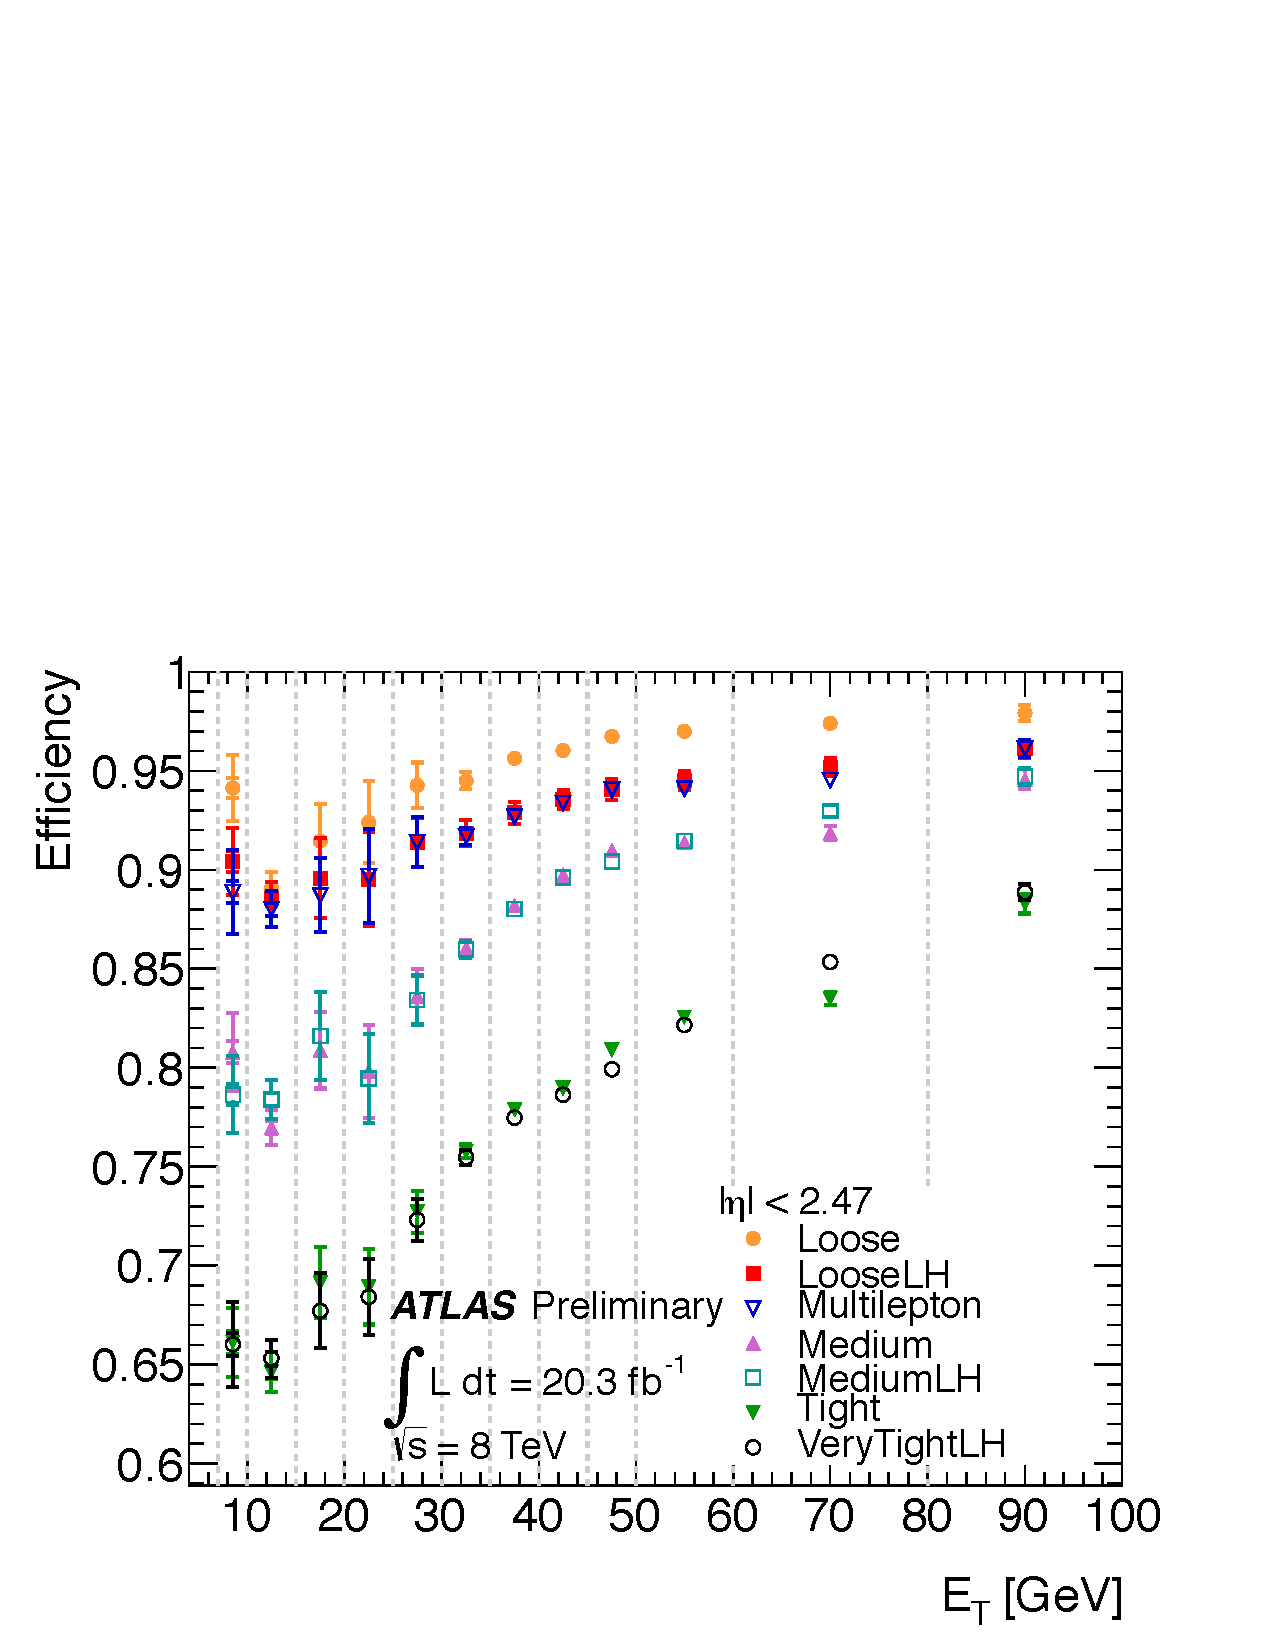
\includegraphics[width=0.4\textwidth]{fig/reconstruction/elec_TP_et.pdf}
    \label{chap:reconstruction:fig:elec_tp_et}
    }
    \subfigure{
    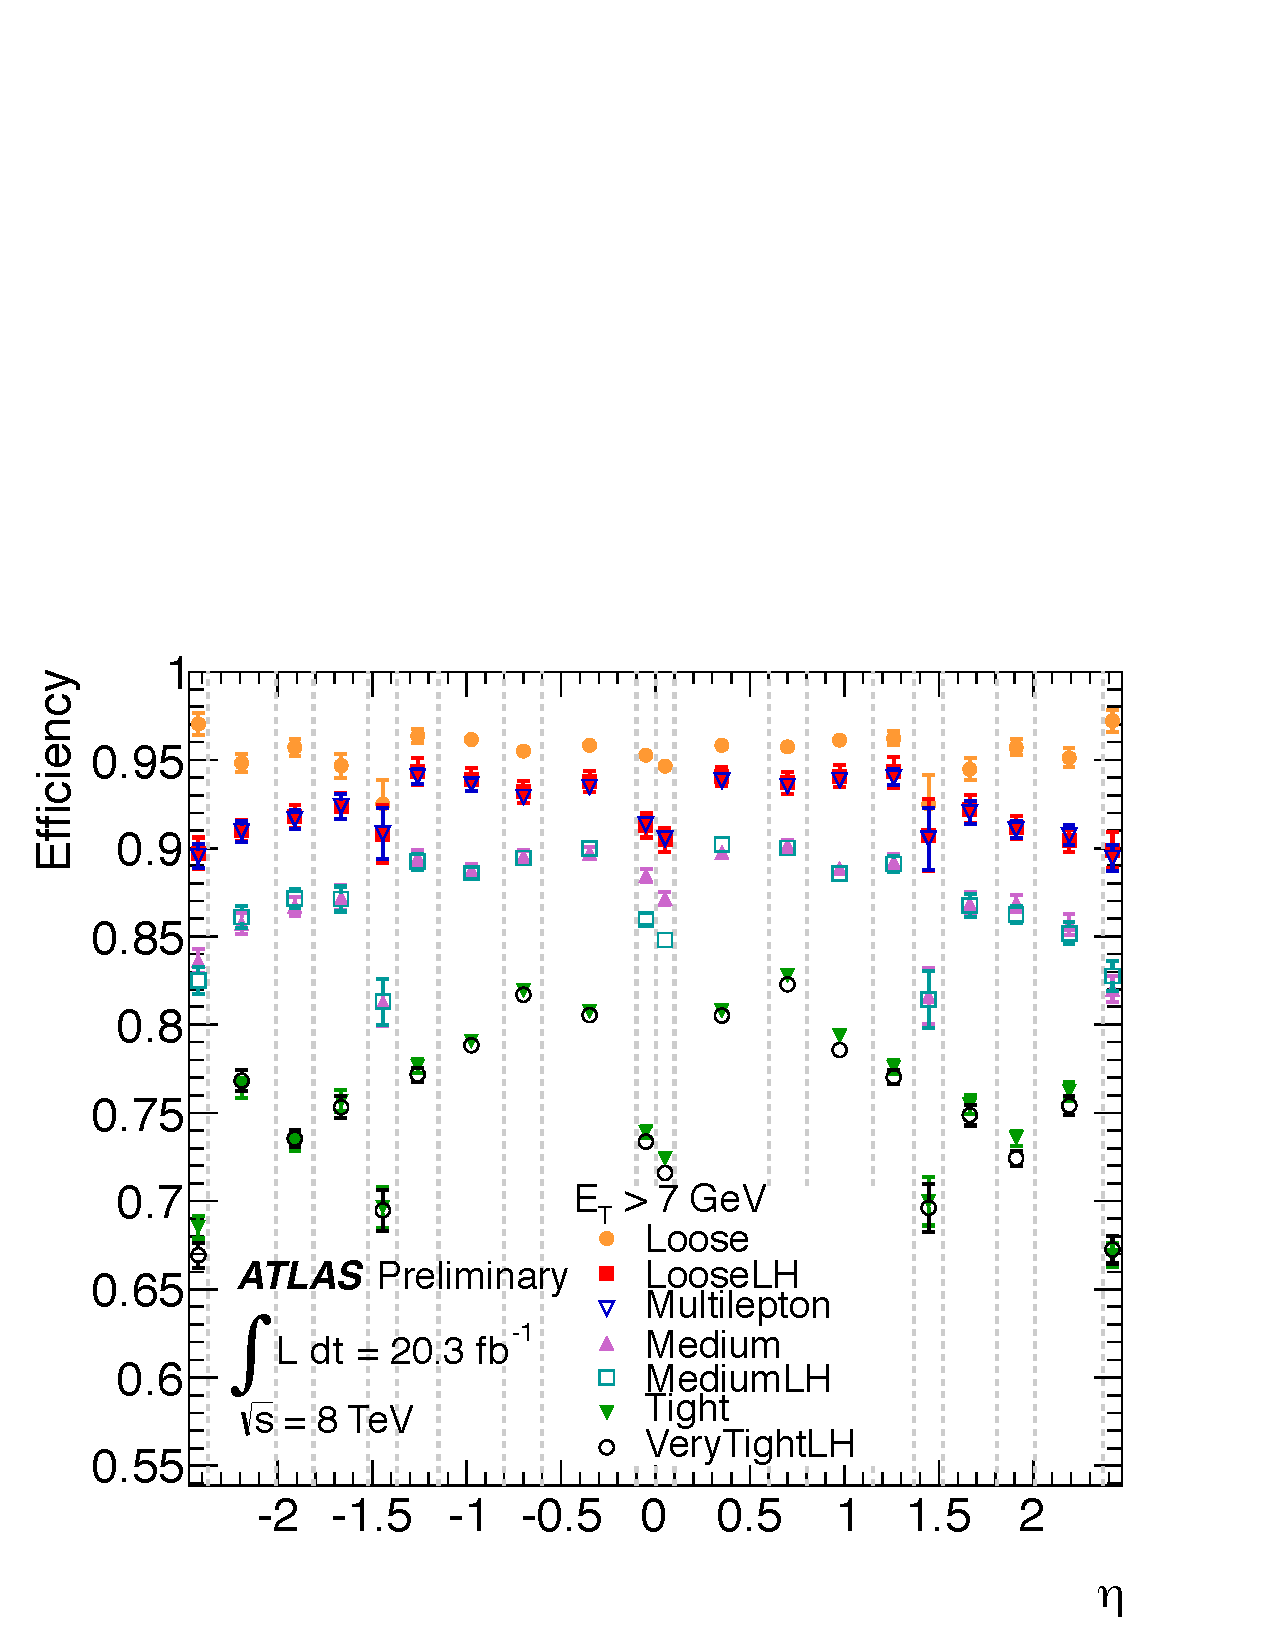
\includegraphics[width=0.4\textwidth]{fig/reconstruction/elec_TP_eta.pdf}
    \label{chap:reconstruction:fig:elec_tp_eta}
    }
    \subfigure{
    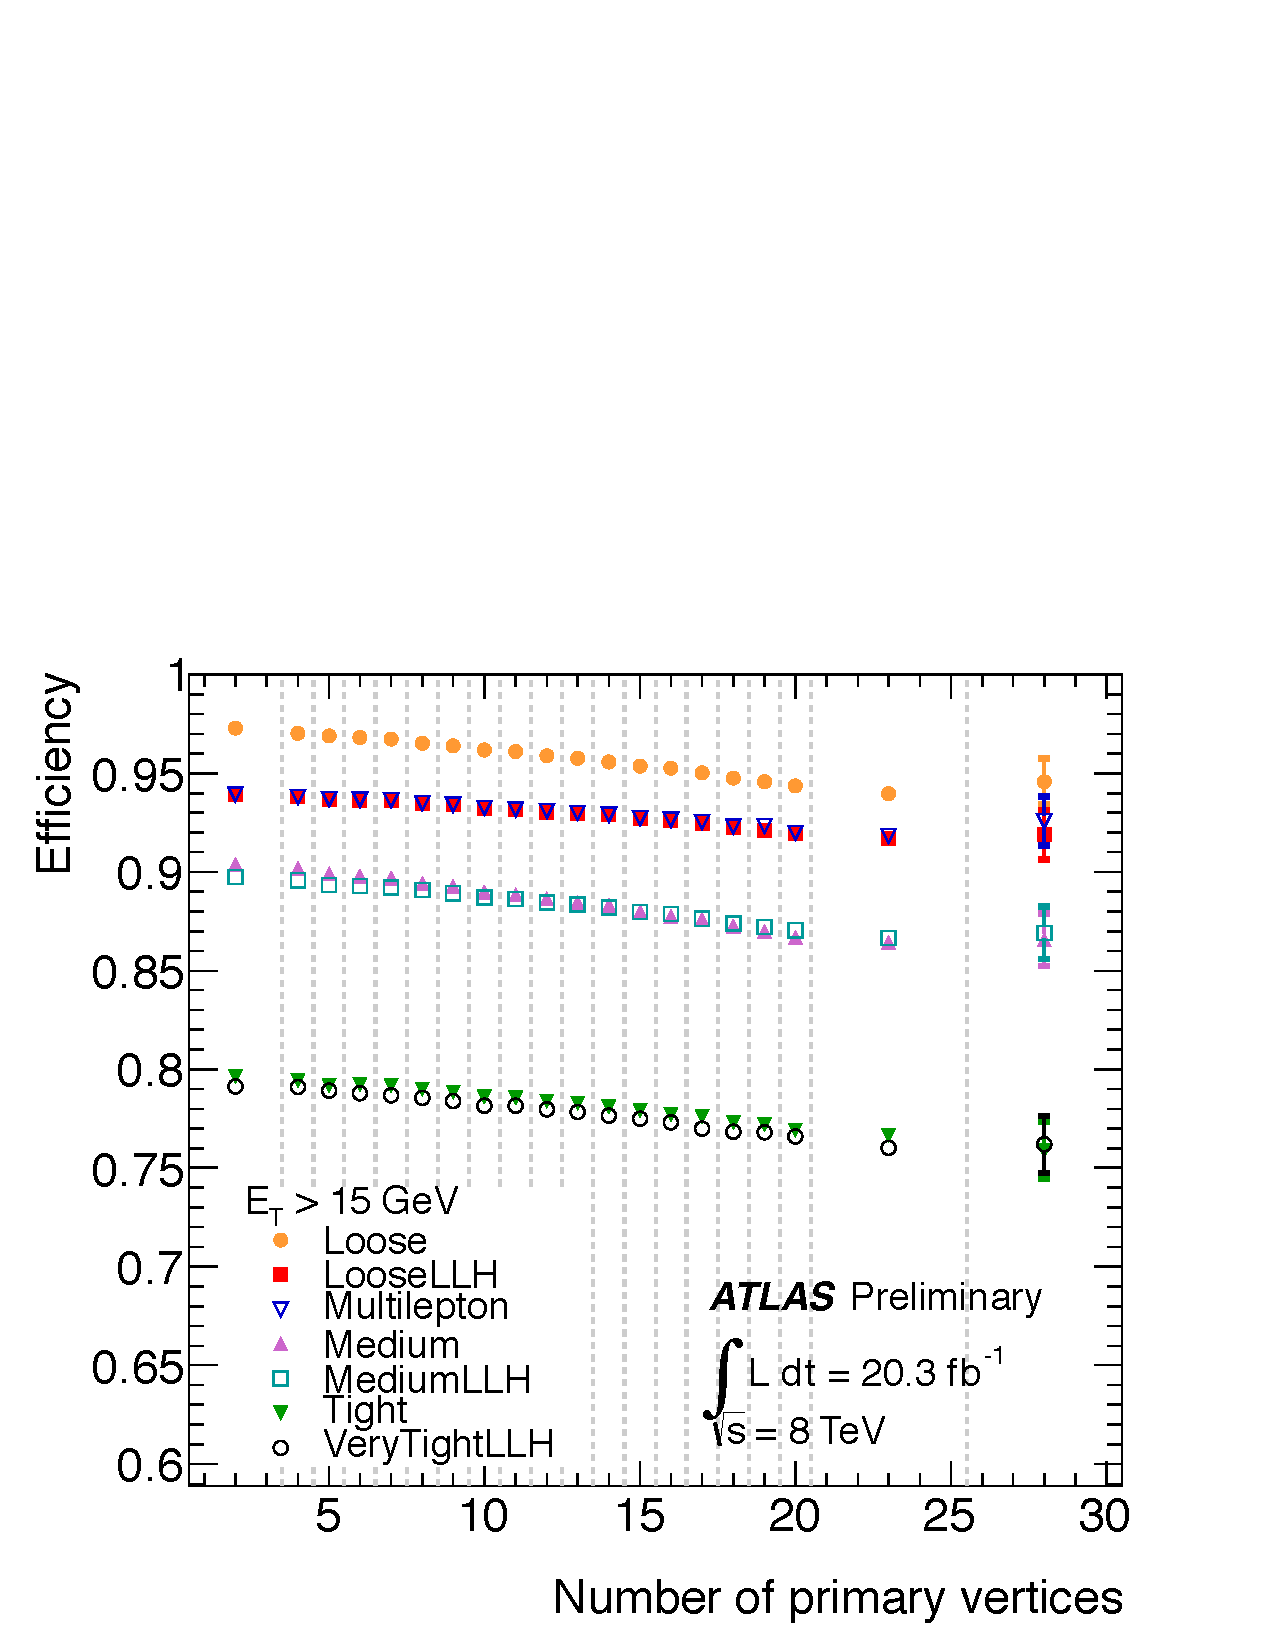
\includegraphics[width=0.4\textwidth]{fig/reconstruction/elec_TP_Npv.pdf}
    \label{chap:reconstruction:fig:elec_tp_npv}
    }
    \caption[]{Electron identification efficiencies for different
      cut-based and likelihood categories, binned in electron
      \et~\subref{chap:reconstruction:fig:elec_tp_et} and
      $\eta$~\subref{chap:reconstruction:fig:elec_tp_eta}, as well as
      the number of primary vertices in the
      event~\subref{chap:reconstruction:fig:elec_tp_npv}~\cite{bib:ATLAS-CONF-2014-032}.}
\label{chap:reconstruction:fig:elec_tp}
\end{figure}

The efficiency as measured in data is compared to simulated
\Zee~events. Tag and probe electrons are defined as they are in data,
but in the case of MC, the numerator set is the set of probe electrons
that fall within $\Delta{R} < 0.2$ of a true electron in the
simulation. The resulting efficiencies from MC are compared to those
of data, and the ratio of data to MC is computed as a correction which
is applied to MC. These ``scale factors'' are applied to each electron
identified in the event as a function of \et~and $\eta$.

In order to assess the uncertainties on the efficiency measurement--
and the associated scale factors-- several alternative measurements
are carried out. In addition to using the $Z$ peak to select
denominator electrons, a calorimeter isolation variable is used to
select denominator electrons and normalize the background
templates. Moreover, the width of the $Z$ mass window is varied, and the definition
of the tag electron is varied. In total, there are 90 systematic
variations on the efficiency measurement, with the central efficiency
set to the average and the systematic uncertainty the RMS. 
